\normalfont\normalsize
\chapter{Hardware Platform}

In this chapter we will present the hardware platforms used. 


Because we wanted to emphasise not only a new way of aquiring data, but also a simple and low cost one, we have selected The Parrot AR.Drone 2.0 as the work horse that will carry the gateway that will communicate with the nodes from our Sparrow Family . 


chesti ..... help .. anybody

 

\section{The Parrot AR.Drone 2.0}

Parrot AR.Drone is a wifi radio controlled flying quadcopter built by the French company Parrot.
The original drone was released in 2010 and in 2012 it was replaced by version 2.0. Since the launch of the original AR.Drone, more the half a milion units have been sold, making it one of the, if not, the most popular drone on the market.

The reason of its success is not entirely due to the relatively low price of around 300\$ but also because it is very easy to learn how to control the drone and also because of the usb port that accomodate any device using that interface and the linux operating system


\begin{figure}[ht]
\begin{center}
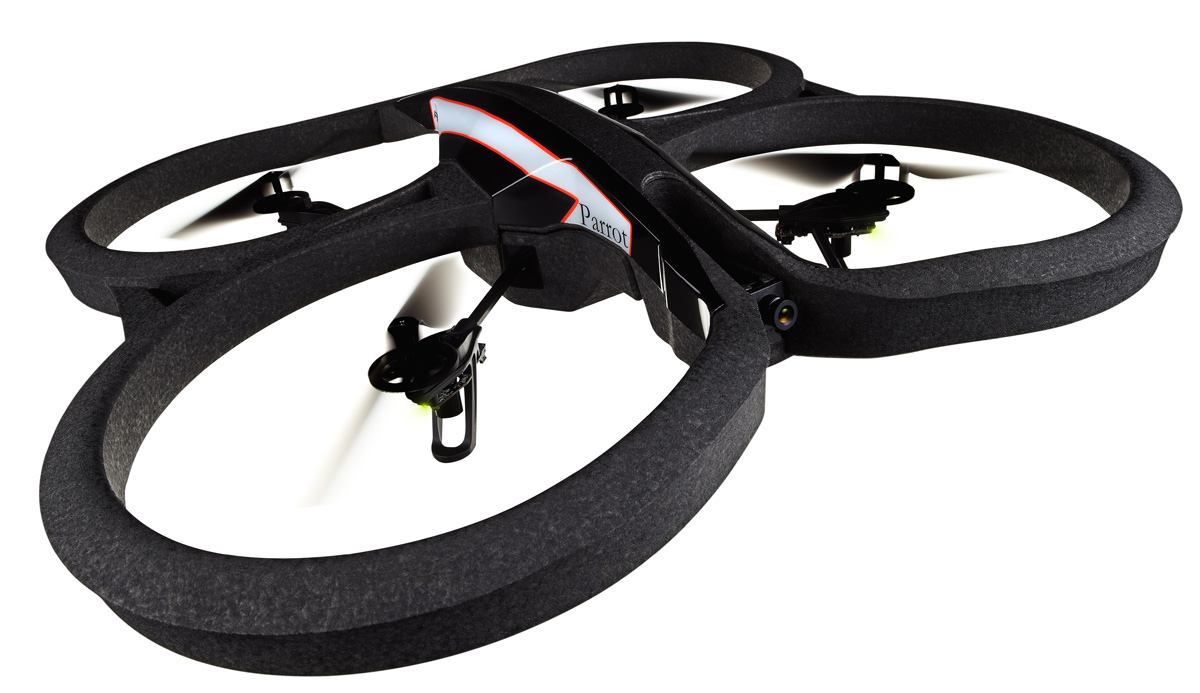
\includegraphics[width=0.9\textwidth]{hw_platform/drone.jpg}
\end{center}
\caption{\small \itshape{The arrot AR.Drone 2.0}}
\end{figure}


Because of those reasons, the Drone has a number of aftermaket modules that can be attached to it like 
the Flight Recorder GPS Module. This module has a built in storage of 4GB for video recording purposes and a built in GPS receiver. This allows the drone to follow a predetermined path of waypoints and to return back from where it took off automatically, all within the limit of the Wi-Fi connection with the control device.
 

The arrot AR.Drone 2.0 specifications are :
\begin{itemize}



\item   1GHz 32 bit ARM Cortex A8 processor with 800MHz video DSP TMS320DMC64x
\item   Linux 2.6.32
\item   1Gbit DDR2 RAM at 200MHz
\item   USB 2.0 high speed for extensions
\item   Wi-Fi b,g,n
\item   3 axis gyroscope 2000°/second precision
\item   3 axis accelerometer +-50mg precision
\item   3 axis magnetometer 6° precision
\item   Pressure sensor +/- 10 Pa precision
\item   Ultrasound sensors for ground altitude measurement
\item   60 fps vertical QVGA camera for ground speed measurement
\item	30 fps 720p front mounted camera 	

\end{itemize}


\section{The Sparrow Family}

\begin{figure}[ht]
\begin{center}
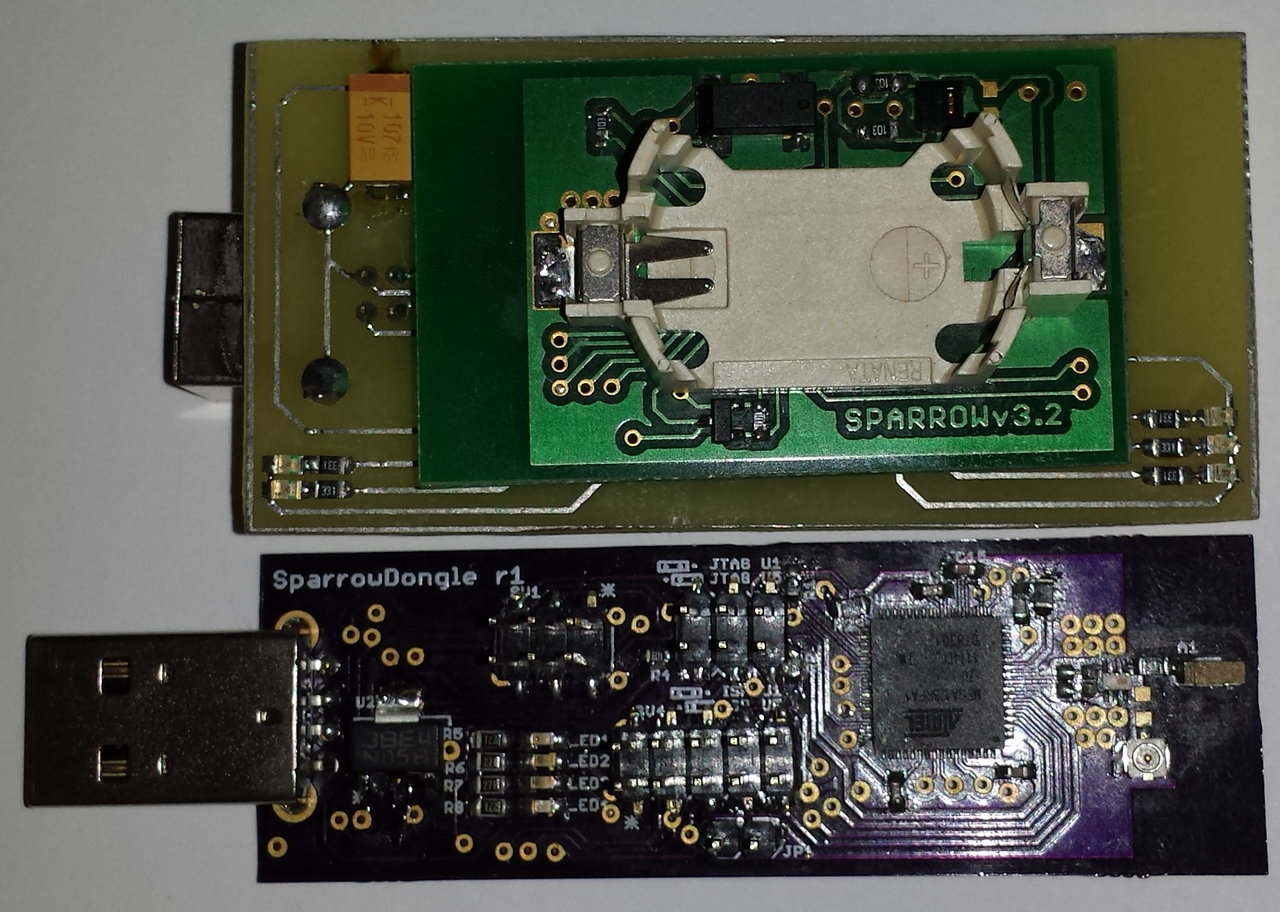
\includegraphics[width=0.9\textwidth]{hw_platform/sparrow.jpg}
\end{center}
\caption{\small \itshape{The Sparrow Dongle next to the SparrowV32}}
\end{figure}
 
The Sparrow Family , composed of the Sparrow Dongle and SparrowV32, use a 2,4 GHz wireless network as a medium of communication. 

At heart,soul and brain of this family lies the ATMega128RFA1. It is an 8bit microcontroller from Atmel that has a very important on-chip 2.4 GHz wireless transceiver that helps in keeping the footprint of the board very small.

The signal received or sent by the wireless transceiver can be boosted by attaching an external atena. For example, in an ideal situation, with no interferences from the outside world , an 8-dbi omni-directional antenna mounted on both communication devices would amount to an around 200 meters of communication range, well over the 70 meters measured with the default antennas.

\subsection{The Sparrow Dongle}

\begin{figure}[ht]
\begin{center}
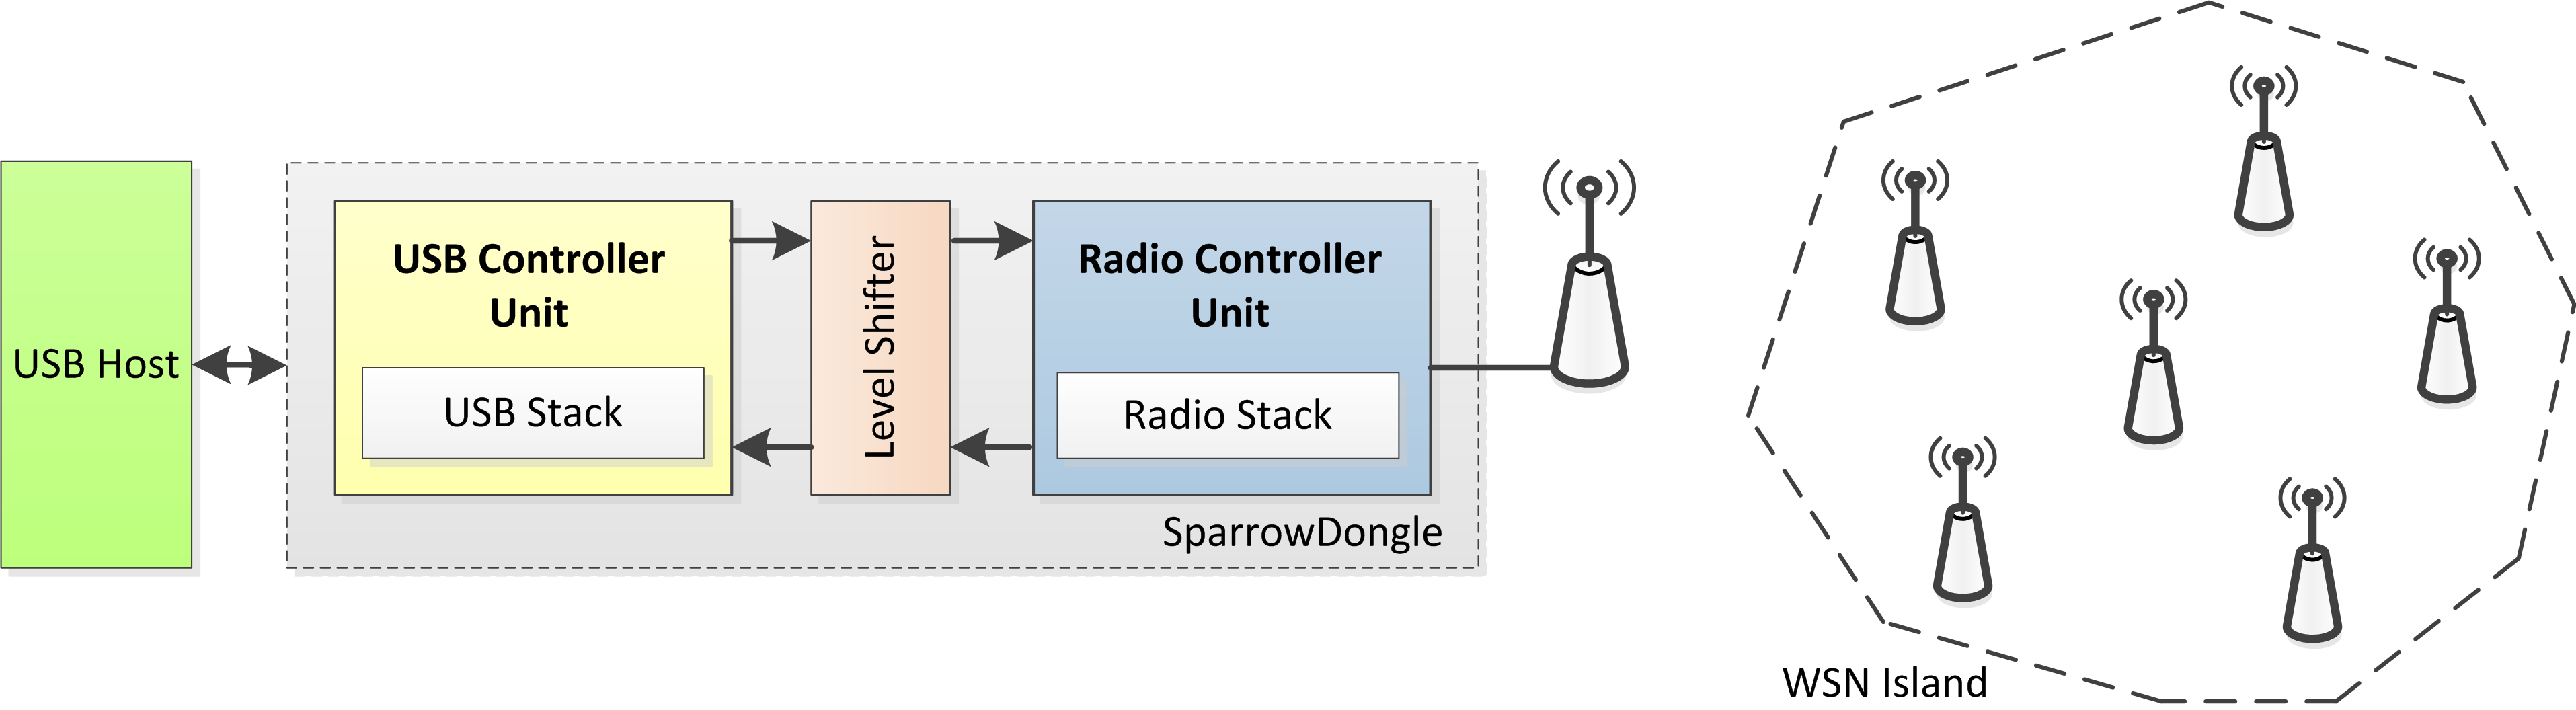
\includegraphics[width=0.9\textwidth]{hw_platform/donge_architecture.png}
\end{center}
\caption{\small \itshape{SparrowDongle stick architecture}}
\end{figure}

The unseen hero of the WSN world, the Sparrow Dongle is the gateway of the Sparrow Family. The Dongle can be connected to any devices that has an usb port and can support USB CDC with ACM module (USB Communications Device Class with Abstract Control Mode). 

The dongle uses Atmega32U4 as a dedicated USB Controller unit. This design allows the RF controller to run any RF communication stack without having the USB code intrude on key timings.


\subsection{The SparrowV32}

\begin{figure}[ht]
\begin{center}
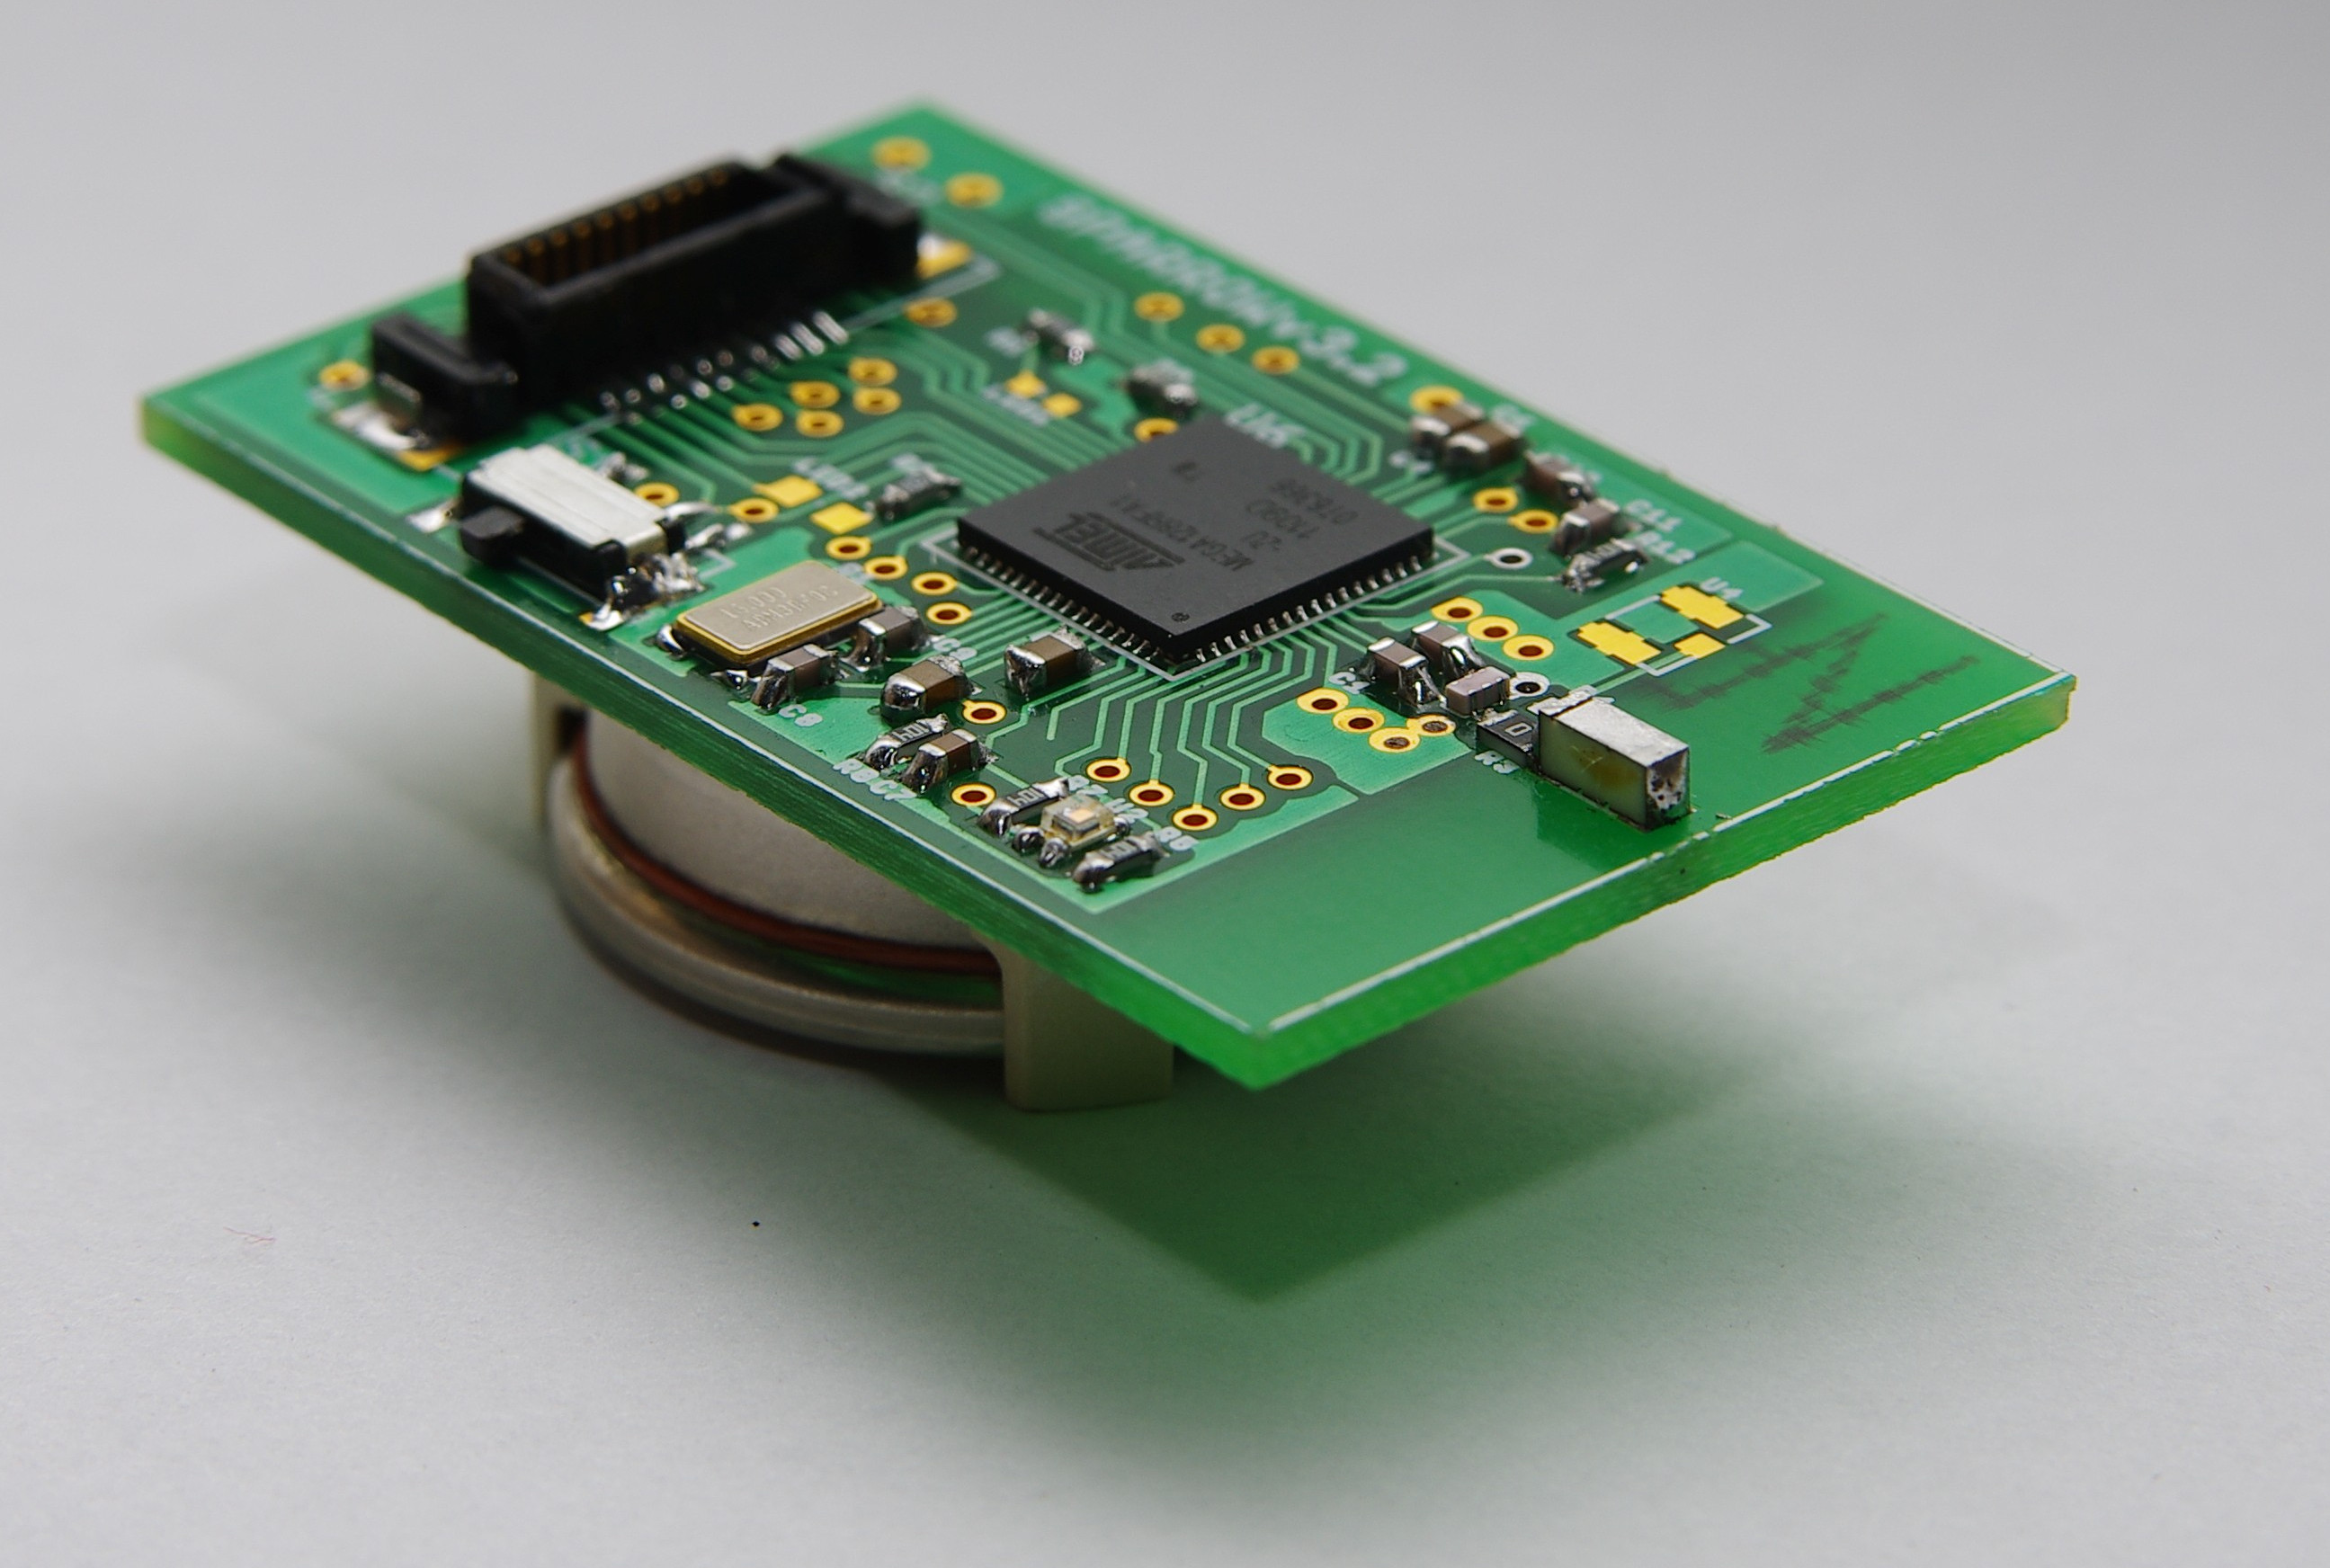
\includegraphics[width=0.9\textwidth]{hw_platform/Sparrowv32.jpg}
\end{center}
\caption{\small \itshape{The SparrowV32}}
\end{figure}


The main hero of The Sparrow Family, the SparrowV32 nodes does all the dirty work of collecting data from the surrounding environment and send it to the Sparrow Dongle. The collected data depends on the sensors of the SparrowV32. The standard implementation has a light, temperature and humidity sensor. Besides this information, it also sends the battery level.
